\documentclass[british]{ntnuthesis}

% \title{Interpretable Machine Learning Models for DAS Data}
\title{Optimizing Big Data Anomaly Detection: Parallel Processing of Geophysical Data and Scalable Autoencoder Models}
\shorttitle{Anomaly Detection on Multidimensional signal data using Unsupervised Learning}
\author{Jørgen Aleksander Fagervik \\
        Supervisor: Ole Jakob Mengshoel}
\shortauthor{J. A. Fagervik}
\date{CC-BY \ntnuthesisdate}

\addbibresource{thesis.bib}


% From https://www.overleaf.com/learn/latex/Glossaries

\makeglossaries % Prepare for adding glossary entries

\newglossaryentry{julia}
{
        name=Julia,
        description={Is an all-purpose programming language specially suited for
scientific computing}
}

\newglossaryentry{python}
{
        name=Python,
        description={Is an all-purpose general programming language suited for scripting, data-science and web applications}
}

\newglossaryentry{llvm}
{
        name=LLVM,
        description={Low Level Virtual Machine, better known as LLVM, is a project trying to provide a modern, SSA-based compilation strategy capable of supporting both static and dynamic compilation of arbitrary programming languages \cite{llvm}}
}

\newglossaryentry{fftw}
{
        name=FFTW,
        description={Fastest Fourier Transform in the West is one of the most famous implementations of the \acrshort{dft} algorithm. It is specialized for running on \acrlong{cpu}s}
}

\newglossaryentry{relu}
{
    name=ReLU,
    description={Rectified Linear Unit is one of the most commonly used activation functions within \acrshort{dnn}s}
}

\newglossaryentry{bibliography}
{
        name=bibliography,
        plural=bibliographies,
        description={A list of the books referred to in a scholarly work,
typically printed as an appendix}
}

\newglossaryentry{maths}
{
    name=mathematics,
    description={Mathematics is what mathematicians do}
}
\newglossaryentry{pubdas}
{
    name=PubDAS,
    description={A PUBlic Distributed Acoustic Sensing Datasets Repository for Geosciences}
}

\newglossaryentry{idun}{
    name=IDUN,
    description={The Idun cluster is a project between NTNU's faculties and the IT division that aims at providing a high-availability and professionally administrated compute platform for NTNU}
}

\newglossaryentry{svm}
{
    name=Support Vector Machine,
    description={Common machine learning technique}
}




% --------------------
% ----- Acronyms -----
% --------------------

\newacronym{ntnu}{NTNU}{Norwegian University of Science and Technology}
\newacronym{ai}{AI}{Artificial Intelligence}
\newacronym{ast}{AST}{Abstract Syntax Tree}
\newacronym{mb}{MB}{Megabyte}
\newacronym{gb}{GB}{Gigabyte}
\newacronym{tb}{TB}{Terrabyte}
\newacronym{ml}{ML}{Machine Learning}
\newacronym{fft}{FFT}{Fast Fourier Transform}
\newacronym{rfft}{RFFT}{Fast Fourier Transform for Real Numbers}
\newacronym{dft}{DFT}{Discrete Fourier Transform}
\newacronym{mpi}{MPI}{Message-passing interface}
\newacronym{ram}{RAM}{Random-access memory}
\newacronym{gcd}{GCD}{Greatest Common Divisor}
\newacronym{hpc}{HPC}{High Performance Computing}
\newacronym{api}{API}{Application programm interface}
\newacronym{gpu}{GPU}{Graphics processing unit}
\newacronym{tpu}{TPU}{Tensor processing unit}
\newacronym{cpu}{CPU}{Central processing unit}
\newacronym{das}{DAS}{Distributed accoustic sensoring}
\newacronym{ann}{ANN}{Artificial neural network}
\newacronym{cnn}{CNN}{Convolutional neural network}
\newacronym{rnn}{RNN}{Recurrent Neural Network}
\newacronym{dnn}{DNN}{Deep Neural Network}
\newacronym{repl}{REPL}{Read-eval-print loop}
\newacronym{lstm}{LSTM}{Long short-term memory}
\newacronym{jit}{JIT}{Just-in-time}
\newacronym{hdf}{HDF}{Hierarchical Data Format}
\newacronym{hdf5}{HDF5}{Hierarchical Data Format version 5}
\newacronym{sisd}{SISD}{Hierarchical Data Format version 5}
\newacronym{simd}{SIMD}{Single instruction, multiple device}
\newacronym{misd}{MISD}{Multiple instructions, single device}
\newacronym{mimd}{MIMD}{Multiple intstructions, multiple device}
\newacronym{spmd}{SPMD}{Single program, multiple device}
\newacronym{cgf}{NTNU CGF}{NTNU Centre for Geophysical Forecasting}
\newacronym{posix}{POSIX}{Portable Operating System Interface}
\newacronym{asn}{ASN}{ALCATEL SUBMARINE NETWORKS}
\newacronym{dsp}{DSP}{Digital Signal Processing}
\newacronym{adam}{ADAM}{Adaptive Moment estimation}
\newacronym{sgd}{SGD}{Stochastic Gradient Descent}
\newacronym{gru}{GRU}{Gated Recurrent Unit}
\newacronym{llm}{LLM}{Large Language Model}
\newacronym{sota}{SOTA}{State of the Art}
\newacronym{dl}{DL}{Deep Learning}
\newacronym{vae}{VAE}{Variational Auto Encoder}
\newacronym{mae}{MAE}{Mean Absolute Error}
\newacronym{mse}{MSE}{Mean Squared Error}
\newacronym{gan}{GAN}{Mean Squared Error}
\newacronym{dbscan}{DBSCAN}{Density-Based Spatial Clustering of Applications with Noise}
\newacronym{adagrad}{AdaGrad}{Adaptive Gradient Algorithm}
\newacronym{fir}{FIR}{Finite Impulse Response}
\newacronym{roi}{ROI}{Range of Interest} % add glossary and acronym lists before document
\usepackage{listings}
\usepackage[table,xcdraw]{xcolor}
\usepackage{siunitx}
\usepackage{multirow}
\usepackage{pgfplots}
\usepackage{textcomp}


\usepackage{caption}
\DeclareCaptionFont{white}{\color{white}}
\DeclareCaptionFormat{listing}{\colorbox{gray}{\parbox{\textwidth}{#1#2#3}}}
\captionsetup[lstlisting]{format=listing,labelfont=white,textfont=white}

% Define Julia style
\lstdefinelanguage{Julia}{
  keywords={abstract, break, case, catch, const, continue, do, else, elseif, end, export, false, for, function, global, if, import, in, macro, module, otherwise, quote, return, true, try, using, while, type, mutable, struct, @inline, @simd, @time, @btime, @layer, @functor, @error, @warn, @show, @inbounds, @kwdef, @view, @layout, @gif,
  Real, Integer, Int, Int8, Int16, Int32, Int64,
  String, AbstractString,
  DateTime, Second, Minute, Hour, Date,
  Bool, Tuple, Matrix, Dict, Set, Vector, AbstractArray, AbstractVector, AbstractMatrix,
  AbstractFloat, Float, Float8, Float16, Float32, Int64,
  },
  sensitive=true,
  comment=[l]\#,
  morecomment=[s]{\#=}{=\#},
  morestring=[b]",
}

\definecolor{backcolour}{rgb}{0.99,0.99,0.99}
\definecolor{codegreen}{rgb}{0,0.6,0}

% Define a custom style
\lstdefinestyle{dasstyle}{
    backgroundcolor=\color{backcolour},   
    commentstyle=\color{codegreen},
    basicstyle=\ttfamily\footnotesize,
    breakatwhitespace=false,         
    breaklines=true,                 
    keepspaces=true,                 
    numbers=left,
    frame=single,
    numbersep=5pt,                  
    showspaces=false,                
    showstringspaces=false,
    showtabs=false,                  
    tabsize=2,
}

% Use \lstset to make myStyle the global default
\lstset{style=dasstyle}

\begin{document}


\begin{titlepage}
\newgeometry{left=1.6in, right=2in}
\vspace*{1.5cm}

\noindent  \textcolor{gray}{\large Jørgen Aleksander Fagervik} \\
\vspace{1cm}

\noindent \textbf{\Large Optimizing Big Data Anomaly Detection: Parallel Processing of Geophysical Data and Scalable Autoencoder Models} \\
\vspace{0.5cm}

\noindent {\large A case study on Unsupervised Learning for Anomaly Detection on DAS data using Julia} \\



\vspace{7cm}
\noindent Master's thesis in Computer Science \\
Supervisor: Ole Jakob Mengshoel \\
Co-supervisor: Matrin Landrø \\
July 2024 \\

\vspace{0.2cm}
\noindent Norwegian University of Science and Technology \\
Faculty of Information techonolgy and electrical engineering \\
Department of Computer Science (IDI) \\

\begin{figure}[h]
    
\includegraphics[width=0.28\textwidth]{figures/ntnu_basic.png}
\end{figure}
\end{titlepage}
\restoregeometry
\myemptypage 

\chapter*{Preface}

The beginning of the end. Six years have gone since I started university to pursue my passion. Little did I know what this years would hold, all the friends and people I'd meet, and all the new information I'd learn. I want to reminisce a bit about my journey towards where I am today. \\

I'd like to start off by saying that these years has had me feeling all kinds of emotion. From the happiest moments to the darkest of days. In the end I'm finishing my degree not only as a more proficient engineer, researcher and developer, but also as a more informed and well of human being. \\

I decided ot study computer science at the age of 12. I started of with simple webdesign and Python development, but also dabbled in game programming with the Unity engine. I became a part of Revolve NTNU during my first year, where I learnt a lot, not only about software tools like Git, JIRA and Confluence for documentation, but also software development as a whole. \\

I didn't exactly know what aspect of computer science I wanted to study, so in the en I forged my own path, trying to bridge the gap between HPC and AI. \\

I decided to 

I want to give a huge

\chapter*{Abstract}

Signal processing and \acrfull{ai} has become .

Parts of this thesis are taken from or based on my submitted project assignment in the subject TDT4501 with the title "Parallel DAS Processing: Julia is all you need".
\chapter*{Sammendrag}

Distribuert akustisk sensing (DAS) har blitt en utbredt teknologi det siste tiåret, men de nåværende metodene for prosessering og anomalideteksjon prioriterer ofte nøyaktighet fremfor effektivitet. Denne oppgaven tar for seg utfordringen med å effektivt prosessere DAS-data samtidig som man opprettholder effektive evner for anomalideteksjon. Vi undersøker parallellprosesseringsmetoder for storskala, tettprøvet DAS-data og utforsker anvendelsen av kompakte autoenkodere for rask anomalideteksjon.

Vi presenterer to verktøy: Judas, en pakke for effektiv innlasting og prosessering av DAS-data, og TinyDAS, et skalerbart rammeverk for opplæring av autoenkodere og utføring av anomalideteksjon. Disse verktøyene har som mål å redusere databehandlingsressurser og prosesseringstid betydelig for håndtering av DAS-data. Vi validerer disse programmene ved å bruke både proprietære og åpne DAS-datasett, med fokus på overvåking av jernbane og jordskjelvdeteksjon.

Vår forskning viser at minnekartlegging kan redusere minnekravene for DAS-databehandling betraktelig. I motsetning til eksisterende metoder som laster hele datasett inn i minnet, benytter vår teknikk distribuert binær filsplitting og behovsstyrt innlasting, noe som muliggjør effektiv håndtering av storskala DAS-data med minimal minnebruk. Videre viser vi at inferens i halv presisjon på en kompakt konvolusjonsbasert autoenkoder med bare 46k parametere kan oppdage anomalier i store matriser med 86\% nøyaktighet på bare 5,5 ms.

Dette arbeidet fremmer mer effektive teknikker for behandling av DAS-data, noe som kan være til nytte for ulike bransjer som benytter DAS-teknologi, inkludert infrastrukturovervåking og geofysisk prognosering. Ved å forbedre databehandlingsmetoder og fremme effektivt design av autoenkodere, baner vårt arbeid ved NTNU Senter for Geofysisk Prognosering vei for mer utbredte og ressursvennlige anvendelser av DAS-teknologi i sanntidsscenarioer.



\tableofcontents
\listoffigures
\listoftables
\lstlistoflistings

\printglossary[type=\acronymtype] % Print acronyms
\printglossary                    % Print glossary

\chapter{Introduction}
\label{chap:introduction}

In this very first chapter, we set up the rest of this thesis. We cover our moitvation for this projects, our goals and research questions, what contributions this paper have given as well as an outline for this thesis.

\section{Motivation}

Digital signal processing has over the last 100 years gone from almost non-existent to utmost critical importance. By processing signal data, one can get access to all kinds of information, music, movement and locations. There are tons of different devices for recording signals from the environments. From more well known ones such as microphones and sensors, to less commercial technologies.

The world of digital signal processing is nothing new to academia, and computer science in general. Some of the most magnificent and trailblazing algorithms, like the \acrfull{dft} algorithm revolve around solving problems revolving around these data. With more and more sensors being used around us, as well as the increasing amount of data stored, the larger the need for processing and interpreting this data has become. 
\acrfull{das} is a rather new technology that allows for real-time analysis over fiber-optical cables, and gives us highly sensitive senor data to work with. \acrshort{das} has gained more recognition. \\

It is hard to underestimate the impact \acrshort{ai} has had upon the general population this last couple of years. Ever since OpenAI released ChatGPT the 30th of november 2022 \cite{chatgpt} the amount of \acrshort{ai} technology and applications has exploded, not only large language models (\acrshort{llm}), but other domains have garnered attention as well. \acrshort{llm}s made \acrfull{rnn} more popular than they had been for a while. These models are good at remembering information, making current desicions based on previous ones. \\ 

\acrshort{das} technology in itself has now started garnering attention for research, and several papers have previously studied  how one can process this data. \acrshort{ai} and \acrshort{ml} models have been constructed for looking at time series data, and analyzing sensor data, although several of theses have studied .  Only recently has \acrshort{ai}

Anomaly detection on \acrshort{das} data 

Unsupervised learning has in later years returned after the explosion of generatiive models. They are well suited for detecting novel anomalies \cite{wei2022lstmautoencoder} \cite{srivastava2016unsupervised} and do not require labeling of data, something that can rather dificult on DAS data. Both GANs, AE, and LSTM VAE have been proven to have good metrics for determining anomalies. 


Python has for a long been the \textit{de-facto standard} language both for \acrshort{ai}, \acrshort{ml} and data analysis. All kinds of heavy pre-processing of data before training the data is being written in C or C++ or other more performant languages.    




Previous work on this data (see \cite{projthesis}) revolved around processing \acrshort{hdf5} files as fast and efficient as possible, trying to parallellize already existent code, and take advantage of newer technologies, such as Julia.

\subsection{NTNU SFI Center for Geophysical Forecasting}



We hereby present \texttt{JudasNET}, a LSTM VAE network written in Julia for anomaly detection on \acrshort{das} data. Additionally, we present \texttt{Judas - (Julia \& DAS)}, a Julia package containing functions for parsing HDF5 files, signal processing methods specifically for DAS sensor data, as well as functions for training, inference and utilities for AI models related to DAS data. As a sideeffect, we also show how Julia can be used effectively within multiple different fields to enable , and be easily tuned to their needs,
\section{Goals}

Given the vast scope and multiple facets of our project, it is important to clarify the specific objectives we aim to achieve with this thesis. Our goals are as follows:

\begin{enumerate}
    \item \textbf{Evaluating Julia for Big Data Science Applications}: Determine whether Julia is a suitable programming language for big data, data science and \acrshort{ai} applications
    \item \textbf{Assessing Autoencoders for Anomaly Detection in \acrshort{das} Data}: Evaluate the effectiveness of autoencoders in detecting anomalies within \acrshort{das} data, both in online and offline data.
    \item \textbf{Open Source Contributions for \acrshort{das}}: Contribute to the open-source community, particularly with tools and resources that are beneficial to members of \acrshort{cgf}.
\end{enumerate}


\subsection{Research Questions}

In addition to our goals, the following are a set of research questions we want answers to by the end of the thesis:

\begin{enumerate}
    \item \textbf{Scalability and Parallelization in \acrshort{das} Data Processing}: Can we develop a program that is both scalable and parallelizable for processing and training large \acrshort{hdf5} files?
    \item \textbf{Float16 Processing on \acrshort{das} data}: Can we reduce the precision of \acrshort{das} data to enable faster model training and inference without sacrificing performance?
\end{enumerate}

\section{Research Questions and Contributions}
\label{intro:contribs}

The following list provides the research questions of this thesis: 

\begin{enumerate}
    \item How do the spatial characteristics of \acrshort{das} data impact the performance of autoencoders for anomaly detection?
    \item What autoencoder architectures are most effective for anomaly detection in \acrshort{das} data when computational resources can be limited?
    \item What preprocessing techniques can optimize the efficiency-accuracy trade-off in anomaly detection of \acrshort{das} data?
\end{enumerate}

In this thesis, we study processing and autoencoder-based anomaly detection using \acrshort{das} data. Our work has led to several contributions, including:

\begin{itemize}
    \item \textbf{Autoencoder based anomaly detection}: We compare the effectiveness of different autoencoders for anomaly detection on dense \acrshort{das} data. In particular, we explore the spatial characteristics of in \acrshort{das} data.
    \item \textbf{Julia for data science and \acrshort{ai}}: We evaluate Julia as a programming language for developing high-performance applications and \acrshort{ai} programming.
    \item \textbf{Software}: The following software has been produced as a part of this thesis:
    \begin{itemize}
        \item \textbf{Judas}: A software package developed in Julia for processing \acrshort{das} data. Initially introduced in our project thesis \cite{projthesis}, Judas is now fully operational but only available for members of \acrshort{cgf}. 
        \item \textbf{TinyDAS}: An open-source program written in Python, specifically designed for training and evaluation of autoencoder models, as well as performing anomaly detection on \acrshort{das} data \footnote{\url{github.com/Jafagervik/TinyDAS}}. This program contains code and hyperparameters for 4 different autoencoders.  We establish how Tinygrad \cite{tinygrad} as a software package can be used to create hardware agnostic \acrshort{ai} programs that are scalable across multiple accelerators without changing source code. 
        \item \textbf{JudasNET}: An open-source repository with examples of autoencoders written in Julia \footnote{\url{github.com/Jafagervik/JudasNET}}.
    \end{itemize}
\end{itemize}

Overall, we seek to improve \acrshort{das} data processing and compare the effectiveness of smaller autoencoder models for anomaly detection on this data. In particular, we hope that members of \acrshort{cgf} can use and improve these tools to further \acrshort{das} research.
\section{Thesis outline}

The following list is an outline over the rest of the thesis, and what will be presented for each chapter. \\

%\textbf{Chapter 1: Introduction} - We present the problems, what we want to find out and our motivation for this project. \\

\textbf{Chapter 2: Background and Related Work} - We cover theory regarding \acrshort{das} processing techniques, both relevant \acrshort{dl} architectures and their applications to our problems, as well as some introduction to applicable signal processing techniques. Finally, we discuss relevant literature and work.  \\

\textbf{Chapter 3: Method} - We cover all our practical work and implementation decisions of both programs, including program design, data processing methods, and network architectures. \\

\textbf{Chapter 4: Experiments} - We present our experiments, covering datasets, the experiments scopes, as well as evaluation metrics and experiment setup. \\

\textbf{Chapter 5: Experimental Results} - We present our results from the experiments conducted in the Chapter 4. \\

\textbf{Chapter 6: Discussion} - We discuss the overall findings and results of our experiments. Furthermore, we discuss the current capabilities of our programs, including limitations, and answer our overarching goals. Finally, we discuss both enhancing qualities of the Julia programming language, as well as current limitations within \acrshort{ai} programming. \\

\textbf{Chapter 7: Conclusion and Further Work} - This final chapter concludes our thesis. We conclude our findings and discuss further work. \\

\textbf{Overlap with Project thesis}

Parts of this thesis are based on my submitted project assignment in TDT4501 titled "Parallel DAS Processing: Julia is all you need". Section \ref{met:Judas} is a continuation of previous work conducted in the project thesis \cite{projthesis}. We provide a clear distinction of what has been done before and what's new in regard to Judas (fka. Emerald). Section \ref{met:Julia} is a summarization of an introduction to Julia, previously covered in Section 2.1 of the project thesis. Section "Reflections on Julia" in Chapter 7 covers some of the previous talking points in the project thesis, but the subsection about Julia for \acrshort{ai} programming is new.

\chapter{Background and Theory}
\label{chap:back}

In this chapter, we discuss the underlying theory necessary for our work. That includes \acrshort{ai} and \acrshort{ml} theory, as well as relevant techniques within signal processing. \\

\section{Julia}

Julia is a high performance, dynamically typed programming language created by MIT in 2012, officially released in 2014. It has developed itself into a real alternative to Python, R and MatLab, while outperforming all on them on general benchmarks. As mentioned in \cite{projthesis}, this is mainly due to how Julia is a "Just ahead of time" compiled language. \\ 

Julias fluent type system, accompanied by easy syntax, high performance, \acrshort{repl} tools makes it a great contender for data analysis. We've previously proven how Julia effectively deals with I/O operations, .


DOI \cite{doi:10.1137/141000671}

FLUXXERT
\section{Digital Signal Processing}

The field of \acrfull{dsp} has been researched since the dawn of time. Signals are all around us, and we do have the means to gather and store the data, but how do we process it more efficiently to be able to analyze and interpret the data in a fast and efficient manner.

When working with \acrshort{das} data in particular, we want to filter the data to remove distortion, and get cleaner outputs to work with. A common way to remove signals outside of a range are called High-pass filters and Low-pass filters. 

A high-pass filter is a function that only allows frequencies above a certain threshold to be accepted, while a low-pass filter only accepts frequencies lower than a threshold $T$. A band-pass filter on the other hand, only allows frequencies within a certain range to be accepted.

\begin{figure}[h]
\centering
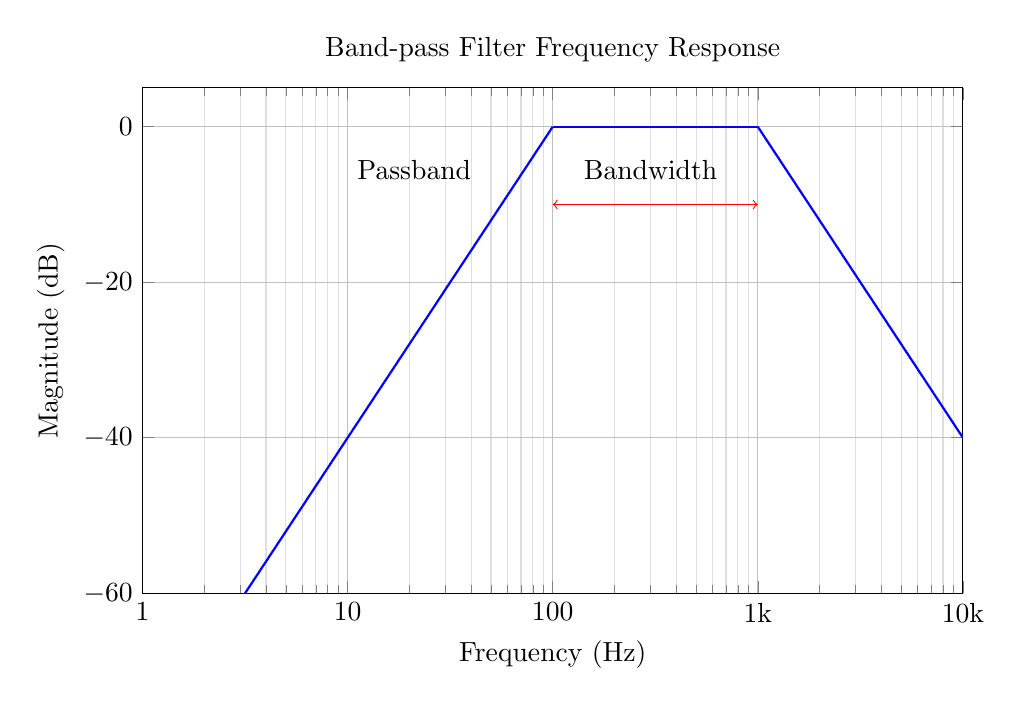
\begin{tikzpicture}
\begin{axis}[
    width=12cm,
    height=8cm,
    xlabel={Frequency (Hz)},
    ylabel={Magnitude (dB)},
    xmode=log,
    xmin=1, xmax=10000,
    ymin=-60, ymax=5,
    xtick={1,10,100,1000,10000},
    xticklabels={1,10,100,1k,10k},
    ytick={-60,-40,-20,0},
    grid=both,
    minor grid style={gray!25},
    major grid style={gray!50},
    title={Band-pass Filter Frequency Response},
]

% Low-frequency rolloff
\addplot[domain=1:100,samples=100,blue,thick] {-40*log10(100/x)};

% Passband
\addplot[domain=100:1000,samples=100,blue,thick] {0};

% High-frequency rolloff
\addplot[domain=1000:10000,samples=100,blue,thick] {-40*log10(x/1000)};

% Annotations
\node[anchor=north west] at (axis cs:10,-3) {Passband};
\draw[<->,red] (axis cs:100,-10) -- (axis cs:1000,-10);
\node[anchor=south] at (axis cs:300,-8) {Bandwidth};

\end{axis}
\end{tikzpicture}
\caption{Ideal Bandpass Filter Response}
\end{figure}


\subsection{Tukey Window}
\label{dsp:tukey}

Window functions are function often used in \acrshort{dsp} and are zero-valued outside of an interval. The Tukey window, also known as the \textit{cosine-tapered window} is one of the more popular window methods, and its mathematical function is described as such: 

\[
    w(x)= 
\begin{cases}
    \frac{1 + \cos{2 \pi \alpha (x + \frac{1-\alpha}{2})}}{2}, & \text{if } x \leq \frac{1-\alpha}{2}\\
    1,              & \text{if } \frac{\alpha}{2} < x \leq \frac{\alpha}{2}\\
    \frac{1 + \cos{2 \pi \alpha (x - \frac{1-\alpha}{2})}}{2}, & \text{if } x > \frac{1-\alpha}{2}
\end{cases}
\]

This window becomes a rectangle when $\alpha = 0$.


\subsection{Resampling}

Also known as sampling-frequency conversion, resampling is the act of modifying the sampling rate of a discrete signal to obtain a new discrete representation of this data. For signal data, lots of samples are usually recorded, but the amount needed to perform calculations or observe patterns does not require this much data. Thus, one can downsample the data to decrease memory usage for storage, as well as time for processing this data. \\


\subsection{Butterworth}

TBI.
\section{Unsupervised Learning}

The major bottleneck of all kinds of machine learning tecniques is data. The more diverse and varied a .

When it comes to \acrshort{ai} and \acrshort{ml} we usually differentiate between tree major types, those being supervised, unsupervised and semi-supervised learning (or self-supervised learning). They differ in the roles that can occur.


\subsection{Linear Layers}

Fully Connected Layer, Dense Layer or Linear Layers  are types of an operation used in several deep learning models. This layer take an input vector and maps it to an output of learnable parameters. The resulting parameters are thus a weight matrix $W$ and a bias vector $b$. It is defined as follows:

\begin{align}
    Y &= XW + b
\end{align}

where:
\begin{align*}
    X & \text{ - input vector [$n x m$] where $m$ is the amount of input features and $n$ is the batch size} \\
    W & \text{ - weight matrix [$m x p$] where $p$ is the amount of output features} \\
    b & \text{ - bias vector of size $p$} \\
    Y & \text{ - output vector [$n x p$]} \\
\end{align*}

Furthermore, an activation function such as \gls{relu} \ref{eq:relu} is applied to the output to achieve nonlinearity.
Lets denote this function as $f$, we now get the following equation.

\begin{equation}
    Z = f(Y) = f(XW+b)
\end{equation}

Linear layers have several advantages, such as computational efficiency, flexibility as well as intrerprebility, where the weight and bias vectors can be interpreted as learned parameters. They also serve as building blocks for other components, such as \acrshort{rnn}s, \acrshort{lstm}s or even attention blocks. \\ 

They are however prone to overfitting and linearity, due to their inherent linearity. They can become quite limited when trying to extract more complex features, thus reducing some of the discriminative power.

\subsection{Parallelism within \acrlong{ml}}

With rapid evolving deep learning architectures, the importance of scalable model training and networks grows larger each year. It is even estimated that these networks grow 1,5x each year \cite{9499913}, making parallelization a vital topic when it comes to \acrlong{ml} to accommodate ever increasing memory needs. Several different hardware accelerators have been created to best accommodate these needs, the most apparent of these are \acrshort{gpu}s. NVIDIA have for several years dominated this market, and their hardware is becoming faster and increasing in memory. \\

By workers, we mainly refer to \acrshort{gpu}s, but this could also be processors or other types of hardware accelerators such as TPUs.


\subsubsection{Model Parallelism}

Deep learning models need to store a lot of data. Weights and biases tend to take up a lot of memory, thus requiring the need of splitting up a model across several workers. As an example, given a model $M$ of 50 layers, we can split this model in 2 parts by having a worker $A$ manage the first 25 layers, and worker $B$ manage the latter half.

The overhead of transferring data across these workers can become a bottleneck, so this should only be utilized when absolutely necessary.

\subsubsection{Data Parallelism}

Data parallelism refers to partitioning data across multiple workers.  Given a large set of data, we can split these data across the workers and store a copy of the model on each worker, calculate gradients across them all and update the trainable parameters for the model. An example of this would be to split a batch of size $b$ across $n$ workers, calculate the gradients and update the model. Before updating the parameters of the model, an average across all parameters is calculated, and each of the copies of the model is updated before continuing.

\subsubsection{Hybrid Parallelism}

This kind of parallelization is a combination of the two previously mentioned techniques. By first splitting a model across several workers, data is subsequently split across multiple workers. 
\section{Anomaly Detection}
\label{back:anomdet}

\textit{Anomaly detection} is about identifying observations that can be deemed inconsistent with the rest of the dataset \cite{anomaly}. These anomalies can also be referred as outliers, surprises, exceptions, depending on domain. Anomaly detection can be used on all kinds of data, ranging from images to time-series data. There are 3 main types of anomalies, and those are \textit{point anomalies}, \textit{contextual anomalies} and \textit{collective anomalies}.

\begin{figure}[!h]
    \centering
    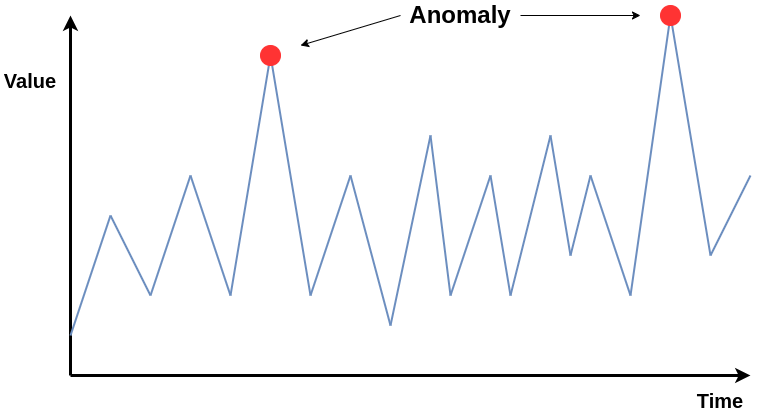
\includegraphics[scale=0.4]{figures/anolay_line.png}
    \caption{Example of anomalies in a time series}
    \label{fig:anomaly_example}
\end{figure}

While point anomalies target single instances that differ from the rest of the dataset, collective anomalies targets groups of instances that together form an anomaly. Contextual ones, as in the word, require context to determine whether or not an anomaly has been detected, and is typically found in time-series data.

Anomaly detection can be performed in a lot of different ways. From common machine learning tasks such as K-means clustering \cite{7507933}, \Gls{svm} \cite{10.1007/978-3-540-28647-9_97}





Given a matrix $a$ of data:

\[
A = \begin{bmatrix}
a_{11} & a_{12} & \cdots & a_{1n} \\
a_{21} & a_{22} & \cdots & a_{2n} \\
\vdots & \vdots & \ddots & \vdots \\
a_{m1} & a_{m2} & \cdots & a_{mn}
\end{bmatrix}
\]

We are interested in finding a region $a_{ij} to a_{kl}$ where $i < k \And j < l$ st. the values within these regions falls outside of the general range


For \acrshort{das} data specifically, anomaly detection can be used for detecting clusters of signals that don't correspond to the predisposed target feature. Registering these outlier signals and receiving real time information about these could prove vital in some cases,  and in best case scenario save lives. 

Dealing with sensitive data 

\subsection{Time series based anomaly detection}

Time series in one dimension is often a great candidate for anomaly detection. Stock market prediction, climate changes and several other series can be used to train networks to recognize point wise anomalies. Layers such as LSTM, RNN and GRU are constructed to store and retrieve information at a later time, thus introducing a memory mechanism. 

\subsection{Image based anomaly detection}

Anomaly detection can also be applied to images. Given a dataset of images with sheep, a image based anomaly detection model would be able to recognize any drastic changes between images. Without the temporal aspect of these problems, convolutional or linear layers are more often used. 

\begin{figure}[!h]
    \centering
    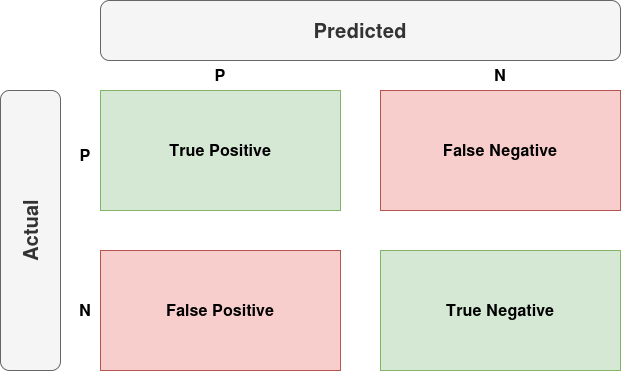
\includegraphics[width=0.5\linewidth]{figures/confmat.png}
    \caption{Caption}
    \label{fig:confmat}
\end{figure}

\section{Recurrent Neural Networks}

\acrfull{rnn}

The main advantage of \acrshort{rnn} 

The building blocks of an \acrshort{rnn} is the recurrant neuron. They take an input $x_t$ at time $t$, with the state at previous time step $h_{t-1}$ and produces the next time step. 

\begin{equation}
    h_t = f(W_hh_{t-1}+W_xx_t)
\end{equation}

RNN have been used witihn geophysical applications before \cite{maulik2020recurrent}. 

Typically, \acrshort{relu} is used as the activation function in these networks, as it is cheap to perform and we don't need more expressive activation functions. Other common activation functions are sigmoid and tanh. 

$$g(z) = max(0, z)$$
$$g(z) = \frac{1}{1 + e^{-z}}$$
$$g(z) = \frac{e^z - e^{-z}}{e^z + e^{-z}}$$

Although RNN has several advantages, they are highly prone to both vanishing gradients as well as exploding gradients. 

Recurrent Batch Normalization
\begin{equation} \label{eq:bnrnn}
    BN(\textbf{h}; \gamma, \beta) = \beta + \gamma \circ \frac{
    \textbf{h} - \hat{E}[\textbf{h}]
    }{
    \sqrt{\hat{Var} [\textbf{h}] + \epsilon}
    }
\end{equation}

\subsection{LSTM - Long Short Term Memory}

One of two more common solutions to avoid the pitfalls \acrshort{rnn}s give us, is to use \acrshort{lstm} cells. 

 As we've mentioned, regular \acrshort{rnn}s struggle with long term memory, something the \acrshort{lstm} cells solves. \\ 


An \acrshort{lstm} cell is built up by the following components: an input gate $i$, a forget gate $f$, a candidate state $g$, an output gate $g$ .
These cells traditionally make use of the sigmoid non-linearity function $\sigma()$

\begin{figure}[h]
    \centering
    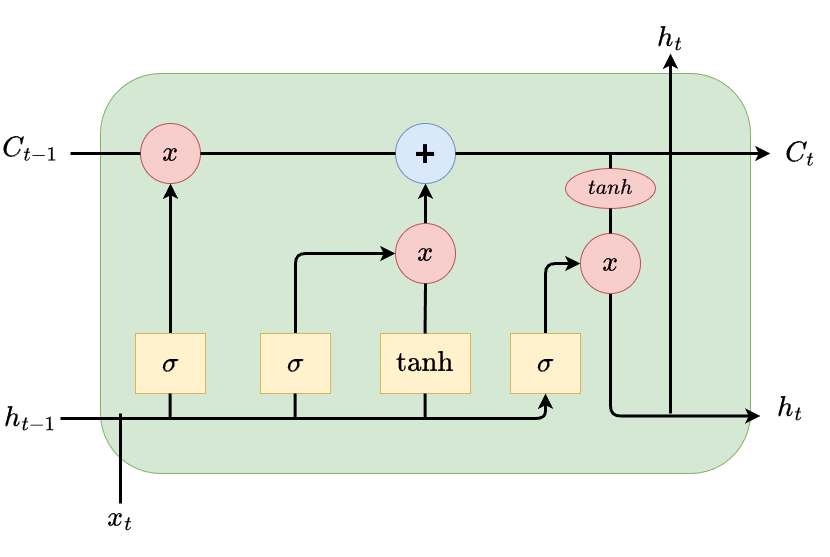
\includegraphics[scale=.4]{figures/lstmcell.png}
    \caption{Example of an LSTM cell}
    \label{fig:lstmcell}
\end{figure}

\begin{figure}[h]
    \centering
    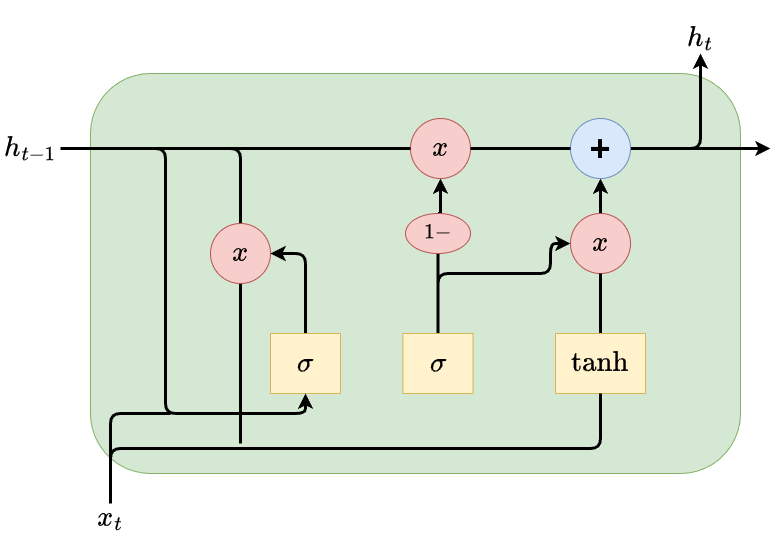
\includegraphics[scale=.4]{figures/grucell.png}
    \caption{Example of an GRU cell}
    \label{fig:lstmcell}
\end{figure}

Compared to the equation for forward pass 

\begin{equation} \label{eq:cnn}
    Y_t = W_xx_t + b
\end{equation}

the \acrshort{lstm} keeps the previous state in mind, thus giving us the equation


\begin{equation} \label{eq:lstm}
    Y_t = W_hh_{t-1} + W_xx_t + b
\end{equation}

Adding batch normalization to this equation and we end up with the following equation \cite{cooijmans2017recurrent}: 

\begin{equation} \label{eq:bnlstm}

c_t = \sigma(\Tilde{\textbf{f}_t} \cdot c_{t-1} + \sigma(\textbf{\Tilde{i}}_t) \cdot tanh(\Tilde{g}_t)
h_t = \sigma(\Tilde{o}_t) \cdot tanh(BN(\textbf{c_t}; \gamma_c, \beta_c))
    
\end{equation}

By applying batch normalization to \acrshort{lstm}s, not only did the models converge faster, the performance was up to par with the unnormalized \acrshort{lstm} \cite{cooijmans2017recurrent}.

Whereas \acrshort{rnn}s shines at \acrshort{nlp}, speech recognition, and media processing, \acrshort{lstm}s is vastly better for time series forecasting due to the memory gates. This makes \acrshort{lstm}s a suitable option for us when working with anomaly detection on sensor data, which in its essence is nothing more than more complex time series data across multiple columns or channels. 

The alternative to using \acrshort{lstm} nodes for our network would be \acrfull{gru}s. Gated recurrent units are ... Simple recurrent units are \cite{lei2018simple}.


\subsubsection{Loss functions on LSMTS}

In typical LSTM 

\acrfull{mae} is the most common algorithm when it 

\subsubsection{KL Divergence}

Another high relevant loss function to look at is the KL divergence  \cite{shlens2014notes}. It is used to measure distance between two probability distributions. Given the prior distribution $P$ and the posterior $Q$, it is described as follows:

\begin{equation}
    \text{KL}(P||Q) = \int_{-\infty}^{\infty} P(x) \log \left( \frac{P(x)}{Q(x)} \right) \, dx
\end{equation}

Regardin variational autoencoders, its objective is to measure discrepancy between the prior and the posterior over latent variables. It has 

The 

\subsubsection{Activation fun}


\subsubsection{Optimizers for Unsupervised Learning }

Diffre



JudasNET uses \Gls{adam} as its optimizer, which is defined as follows: 


\begin{align}
    m_t &= \beta_1 m_{t-1} + (1 - \beta_1) g_t \\
    v_t &= \beta_2 v_{t-1} + (1 - \beta_2) g_t^2 \\
    \hat{m}_t &= \frac{m_t}{1 - \beta_1^t} \\
    \hat{v}_t &= \frac{v_t}{1 - \beta_2^t} \\
    \theta_{t+1} &= \theta_t - \frac{\alpha}{\sqrt{\hat{v}_t} + \epsilon} \hat{m}_t
\end{align}

where:
\begin{align*}
    \theta_t & \text{ - parameters at time step } t \\
    g_t & \text{ - gradient of the loss function at time step } t \\
    \alpha & \text{ - learning rate} \\
    \beta_1, \beta_2 & \text{ - exponential decay rates for the moment estimates} \\
    m_t, v_t & \text{ - first and second moment estimates} \\
    \hat{m}_t, \hat{v}_t & \text{ - bias-corrected first and second moment estimates} \\
    \epsilon & \text{ - small constant to prevent division by zero}
\end{align*}

The original paper sets the following parameters for ADAM: $\beta_1 = 0.99, \beta_2 = 0.9 \mu=10^{-8}$ and $\alpha = 0.001$ \cite{kingma2017adam}.
\subsection{Autoencoder}

The autoencoder is a type of network used to learn efficient encodings of unlabeled data. 

Autoencoders are split into two parts. The encoder $E_\phi$ and the decoder $D_\theta$. The relationship between these can be articulated as such: 

\begin{equation}
E_\phi: X \rightarrow Z 
\end{equation}

\begin{equation}
D_\theta: Z \rightarrow X
\end{equation}

The optima for any kind of autoencoder becomes that of lossless encoding, which can further be described as such:

\begin{equation}
    X = D_\theta(E_\phi(X))
\end{equation}

When a auto encoder is trained to max effiency, we can in some cases remove the decoder part. Since the goal in the beginning was to map data to a lower-dimensional latent space, which has been increased. If ones goal is feature extraction, the decoder is not needed any more. Additionally, by removing the decoder, the overall complexity and size of the model $M$ decreases.


Typical usecases for autoencoders are signal analysis, anomaly detection, reconstructing images and so on. 
One of the more well known usages for autoencoders

\subsubsection{Variational Autoencoder (\acrshort{vae})}

Similar to the regular autoencoder, a \acrfull{vae} also aims to map input over to a feature representation. The diffre. Broadly speaking, the difference between a \acrshort{AE} and a \acrshort{VAE} is that a AE maps inpot to points, where as VAEs map over to a distribution in the latent space. Thus, the \acrlong{vae} can be seemed as a generative model.




VAEs can be trained by backpropagation due to something known as the \textit{reparametrization trick}. We need this because since VAEs maps to a stochastic variable, abckpropagation would else not be feasible.

\begin{align*}
\text{Given:} & \quad \text{Encoder LSTM outputs: } h \\
& \quad \text{Mean vector: } \mu \\
& \quad \text{Log variance vector: } \log(\sigma^2) \\
\text{Sample:} & \quad \epsilon \sim \mathcal{N}(0, 1) \\
\text{Reparameterization:} & \quad z = \mu + \sigma \odot \epsilon \\
\text{Decoder Input:} & \quad z \quad \text{(sampled latent vector)} \\
\text{Training Objective:} & \quad \text{Minimize reconstruction error} \\
& \quad \text{and KL divergence between } q(z|x) \text{ and } p(z) \\
\text{Loss Function:} & \quad \mathcal{L} = \text{reconstruction\_loss} + \text{KL\_divergence}
\end{align*}




\subsubsection{LSTM Variational Auto Encoder}

As we've discussed in \ref{ai:lstm} and \ref{ai:rnn}, these types of networks are well suited for . The issues found with \acrshort{rnn}s, such as long term dependencies, are solved with using \acrshort{lstm}s, and also initializing the weights in a more intelligent way. We are not going to make use of transfer learning for our network, thus we solely rely on \acrshort{lstm}s to solve these issues.

Combining the \acrshort{lstm} with an autoencoder approach, we'll be able to create a network well suited for anomaly detection on variable time series data.

\textbf{KEYS TO GETTING A GOOD VARIATIONAL AUTO ENCODER}

\begin{itemize}
    \item Pick the righ size for the latent space
    \item Learning rate scheduler  and hyperparam tuning 
    \item BETA COEFFICIENT
\end{itemize}

An effort has been made into trying to improve autoencoders for anomaly detection \cite{tan2023improving}

\chapter{Related Work}
\label{chap:relwork}

Signal processing, though nothing new to academia, has a rich and developed history. I 


The most relevant as of now might be \cite{s21196627} which directly looks at  data and deep learning models

\section{Research on AI and DAS data}

Research on signal data isn't really new. 

Seismic DAS using Unet \cite{zhu2023seismic}

\subsection{Research on AI and DAS data}

\chapter{Method}
\label{chap:method}

In this chapter, we go through our choice of language and frameworks for implementation. Furthermore, we go into detail about the datasets we use, how we improve on the previous implementation of our program and how data is processed. Finally we describe how our models are implemented, as well as a choice of parameters and architectures. \\


% Data
\section{Data}

For this project, we will be working with data recorded from BANE-NOR, where a train is travelling between Trondheim and Storen the 31st of august 2021. Data is split between 5000 sensor channels, lasting us a day.
The data is recorded in \acrshort{hdf5} files, with each file containing 20000 samples for 10 seconds, giving us a sample rate of $2000Hz$. The


\begin{table}[h]
\centering
\begin{tabular}{|r|r|r|r|r|}
\hline
\textbf{1}                & \textbf{2}               & \multicolumn{1}{c|}{\textbf{...}} & \textbf{n-1}             & \textbf{n}               \\ \hline
1f-3                      & 2.3f-5                   & 4f-4                              & 3.4f-6                   & 3f-1                     \\ \hline
3f-1                      & 3f-1                     & 3f-1                              & 3f-1                     & 3f-1                     \\ \hline
\multicolumn{1}{|c|}{...} & \multicolumn{1}{c|}{...} & \multicolumn{1}{c|}{...}          & \multicolumn{1}{c|}{...} & \multicolumn{1}{c|}{...} \\ \hline
4f-2                      & 3f-1                     & 3f-1                              & 3f-1                     & 3f-1                     \\ \hline
\end{tabular}
\caption{Table explaining how the table looks like}
\label{fig:datatable}
\end{table}



TODO: Figure over dataflow  

\subsection{Pre processing}

After the data has been loaded \cite{projthesis}, it's still not ready for processing. 

The function \lstinline|process_DAS_data| takes in the signal data, perform a tukey \ref{dsp:tukey} window algorithm over it. We then run a bandpass filter algorithm with Butterworth over it to extract the and 

\begin{figure}
    \centering
    \lstinputlisting{code/procdasdata.jl}
    \caption{Process DAS data function}
    \label{fig:procdasdata}
\end{figure}


After applying a window function and a filter function to combat oscilleration, we're now ready to run an fft over this data. 


The 

\begin{figure}[h]
    \centering
    \includegraphics{figures/banenor_20210831.png}
    \caption{Heatmap of the processed train data during the 31st of august 2021 from Trondheim to Storen}
    \label{fig:trdstrdas}
\end{figure}

\subsection{Data preparation before } 

Now that the data has been successfully pre-processed, we still need to 



\subsubsection{Data augmentation}


\section{Programming Languages and Frameworks}

Our initial decision was to continue using Julia for our \acrshort{dl} methods, and train our models on the same dataset provided by \acrshort{cgf}. We created a Julia package called JudasNET, containing code for training different \acrshort{ai} models. However, due to severe computational limitations, we were unable to continue our work on the previous decision. With only 11GB of VRAM, the single \acrshort{gpu} available quickly became a bottleneck. Not only do we need to store batches of \acrshort{das} data matrices, but we also need to store the weights and biases of our models. By switching to a open source dataset, we would be able to use \Gls{idun}, and leverage multiple \acrshort{gpu}s and in general more computational power. Since the BANENOR dataset is close sourced, we would not be able to train our models on any other resources outside of those provided by \acrshort{cgf}.

Not only were our attempts at training models unsuccessful, Julia's main framework for \acrshort{ml} training \texttt{Flux.jl} does not provide built in tools for multigpu training. \\  

The more obvious choice would now be to use the Python package \texttt{Pytorch}, which is well established, documented and supports not only data parallel training \footnote{  \href{https://pytorch.org/docs/stable/generated/torch.nn.DataParallel.html}{https://pytorch.org/docs/stable/generated/torch.nn.DataParallel.html}}, but also distributed data parallel training \footnote{\href{https://pytorch.org/tutorials/intermediate/ddp_tutorial.html}{https://pytorch.org/tutorials/intermediate/ddp\_tutorial.html}}. What needs to be mentrioned is that Pytorch is heavily optimized for CUDA and NVIDIA \acrshort{gpu}s, and in general performs significantly better on these accelerators, compared to other alternatives such as AMD, NV, METAL and so on. \\ 

We want to create models where we don't need to change much of our code to run on different accelerators. We also want \acrshort{cgf} to  quickly be able to both continue training and running their own models. NVIDIA \acrshort{gpu}s are generally expensive, many of them reaching prices of tens of thousands of dollars per \acrshort{gpu}. We realize that this would not be feasible for \acrshort{cgf} to invest in right now, and thus we decided to look for other frameworks which supports a broader range of hardware accelerators. \\ 

Due to these constraints, we believe Tinygrad \cite{tinygrad} will be a well suited framework for our usecase.

\subsection{TinyGrad}











\mycomment{



DOI \cite{doi:10.1137/141000671}

\subsection{Flux.jl}
\label{back:flux}

Flux is a machine learning library written entirely in Julia released and published in 2018 \cite{Flux.jl-2018, Innes2018}. It allows the user to write their own machine-learning libraries. \acrshort{gpu} support is also native, through the inclusion of \texttt{CUDA.jl} \cite{Besard_2019}. We will be writing all of our models using Flux, or \texttt{Zygote.jl}, which \texttt{Flux.jl} is based on. 

Although \texttt{Flux.jl} is the preferred way to work with \acrshort{ai} in Julia, other prominent alternatives exists as well. \texttt{MLJ.jl} \cite{blaom2020flexible} \cite{Blaom2020} is a framework provided by the Alan Turing Institute\texttrademark, providing interfaces and functions for working with about 200 machine learning models. 

\texttt{Tensorflow.jl} is a Julia package which wraps Tensorflow functions from Python to be able to work with ethem

Julia has support for working on outlier detection as follows: \cite{muhr2022outlierdetectionjl}.

A list of all packages used in addition to Flux.jl can be found in the appendix \ref{app:packages}.

}

We start at the same spot we left off after the project thesis. Before we go on to explain what's been done this semester, lets recap. 

We initially got started by just getting a drive with lots of \acrshort{das} data, and a script from \acrfull{asn} which set up us perfectly. We chose to rewrite python code to a language similar to that of Matlab and Python. We landed on Julia, and with its broad ecosytstem it has support for all kinds of development we'd ever need. \\

We first wrote a 1:1 copy of the script, and then parallelized parts of the code until we had a version that could handle large amounts of data in parallel. We also wrote methods for being able to run a window over and \\ 


\section{Overview}

Our product is split into two apis. Those being \texttt{Judas} and \texttt{JudasNET}. Judas is the direct continuation from \cite{projthesis}
The \acrshort{api} that's being created is called \texttt{Judas} (Julia and DAS) and is split in 3 modules as well as a seperate Utils file as shown in \ref{fig:ccuda}

\begin{figure}[h]
    \centering
    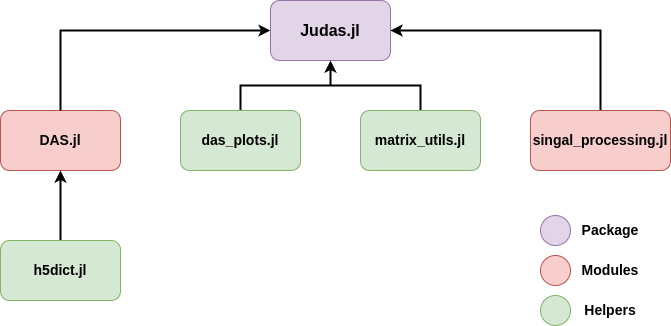
\includegraphics[scale=.6]{figures/judas_overview.png}
    \caption{Overview over our package Judas}
    \label{fig:judasoverview}
\end{figure}

% DAS
\section{Judas - Software Framework}

The DAS folder has not changed much substantially. The main difference from before is how we now instead of writing matrix data to one large binary file, data is split into multiple files, and only read when needed.

Contrary to what was mentioned before, the output of the function \texttt{load\_DAS\_files} has actually changed. Previously, we stored a whole vector of the timestamps for each sample. Not only was this cistly, but actaully totally redundant. If the timestamp of the first row is known, the sampling rate $T$ and which row to look at, one can instead calculate the timestamp like this: 
\lstinline|start_time + MilliSecond(idx * T * 1000)|. This in-place calculation can be done multiple times effectively in Julia using the broadcast operator (.). This ensures that we don't lose essential information before running our data through through the autoencoder

\begin{figure}[h]
\centering
\begin{subfigure}{.5\textwidth}
  \centering
  \lstinputlisting{code/dasstructold.jl}
  \caption{Old DAS Struct}
  \label{fig:olddasstc}
\end{subfigure}%
\begin{subfigure}{.5\textwidth}
  \centering
  \lstinputlisting{code/dasstruct.jl}
  \caption{New Layout for DAS struct}
  \label{fig:newdasstc}
\end{subfigure}
\caption{Comparison between different versions of the DAS struct}
\label{fig:dasstccmp}
\end{figure}




\textbf{API Usage}

\begin{figure}[h]
    \centering
    \lstinputlisting{code/apiusage.jl}
    \caption{How to use our API}
    \label{fig:apiusage}
\end{figure}


\begin{figure}[h]
    \centering
    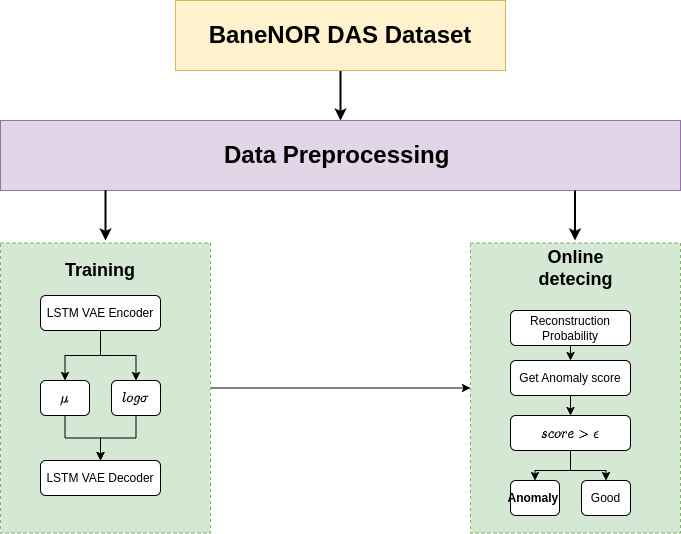
\includegraphics[scale=0.5]{figures/methodflow.png}
    \caption{Dataflow}
    \label{fig:dataflow}
\end{figure}




% NETWORK ARCH
\section{Network Architecture}

The model consists of

\begin{itemize}
    \item Batch size 
    \item skdfj
    \item sdfk
\end{itemize}

\begin{table}[h]
    \centering
    \begin{tabular}{ l c r }
      \hline
      Layer (type) & Output shape & Param \# \\ \hline
      lstm\_1 (LSTM) & (None, 10, 256) & 1234678 \\ \hline
      lstm\_1 (LSTM) & (None, 10, 256) & 1234678 \\ \hline
      lstm\_1 (LSTM) & (None, 10, 256) & 1234678 \\ \hline
      lstm\_1 (LSTM) & (None, 10, 256) & 1234678 \\ \hline
      lstm\_1 (LSTM) & (None, 10, 256) & 1234678 \\ \hline
      Total params: & & \\
      Trainable params: & & \\ 
      Non-Trainable params: 0 & & \\ \hline
      
    \end{tabular}
    \caption{Parameters for our architecture}
    \label{tab:archparams}
\end{table}


\begin{figure}[h]
    \centering
    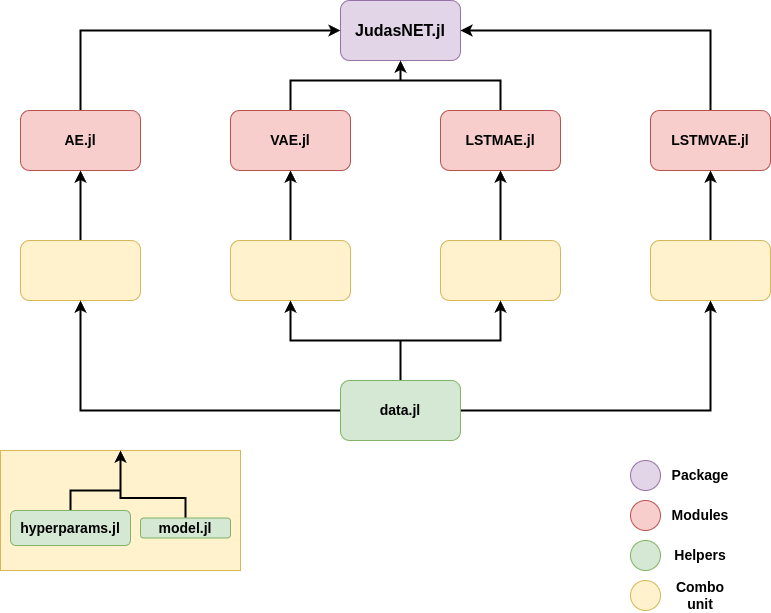
\includegraphics{figures/judasnet.png}
    \caption{JudasNET network architecture}
    \label{fig:judasnet}
\end{figure}


\subsection{Hyperparameters}

See \cite{app:hyperparams} for a detailed view on all the different hyperparameters used for this particular model




\section{SignalProcessing.jl}

After data has been read and processed, it's ready to be processed by signal processing functions 

\section{AI.jl}

The main aspects of this code lies within the module \texttt{AI.jl}. 


\subsection{JudasNET}

\texttt{JudasNET} is the architecture of choice for interpreting data

\begin{figure}{h}
    \centering
    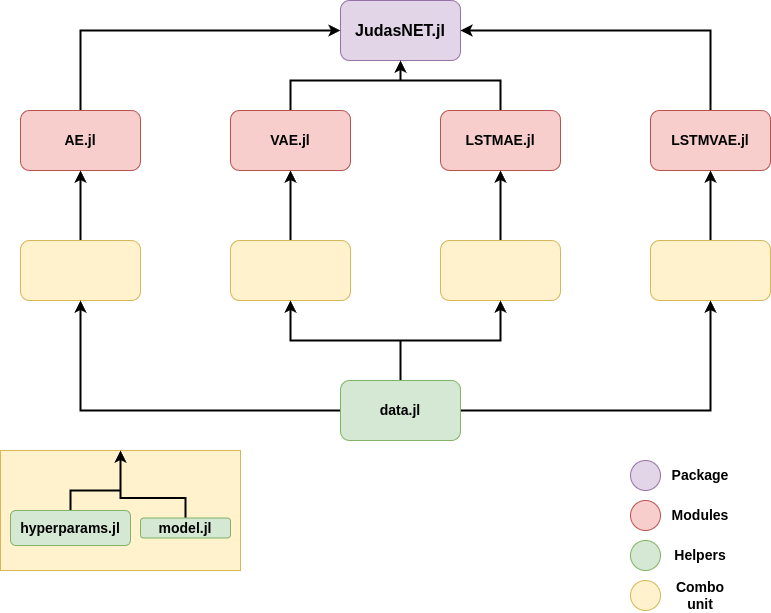
\includegraphics[scale=.6]{figures/judasnet.png}
    \caption{Flowchart over JudasNET}
    \label{fig:judasnet}
\end{figure}

\subsubsection{Modification to Flux.jl}

As mentioned previously, one of the main benefits with Julia packages is the ability to easily add new functionality to packages. When working with \texttt{Flux.jl}, this has certainly been useful. For our research, we had to write our own LSTM functors to be able to achieve a LSTM Autoencoder.  \\

The first of this functors is a regular LSTM, but with \texttt{relu} as the activation function for the different gates. Secondly, we rewrote the TimeDistributed layer \cite{keras} for Flux since there is no corresponding alternative as of the writeday of this paper. The final layer we had to recreate is what's known as a \texttt{RepeatVector} in Keras. When we have all of these together, we can finally put them together and write our model. 

\begin{figure}[h]
    \centering
    \lstinputlisting{code/judasnet.jl}
    \caption{JudasNET flux model}
    \label{fig:fluxjudasnet}
\end{figure}



We're using \acrfull{adam} as the choice of our optimizer

\begin{equation}
    \omega - \alpha \frac{v_{dw}}  {\sqrt{s_{dw}} + \epsilon}
\end{equation}


\section{TinyDAS}

TinyDAS is a program we've created to easily be able to train, and test different types of autoencoder models for anomaly detection. The main ideas behind creating this program are as follows:

\begin{enumerate}
    \item New autoencoder models are easy to add
    \item Easy to tune configurations
    \item Scalable from single core computer to distributed systems.
    \item The program is not tied to any particular hardware accelerator architecture
    \item Support for half precision training
    \item Support for transfer learning and early stopping
    \item Testing of autoencoders should be easy to add
\end{enumerate}

Based on these conditions, our choice of framework was tinygrad \ref{back:tinygrad}, mainly since the framework is designed to be accelerator-independent.

\subsection{\acrshort{api} design}

\subsubsection{Early Stopping}

Even though the model loss ideally should decrease to eventually reach zero almost immediately, this is never the case. Overfitting is when the loss starts increasing, never to return to its best value. To avoid spending time and resources on unnecessary training, we implement a useful mechanism called early stopping, which is described as follows:

\begin{align*}
&\text{Stop at epoch } T \text{ if:} \\
&\forall i \in \{T-p+1, ..., T\}: L_v(i) > L_v^* - \epsilon \\
&\text{where } L_v^* = \min_{j=1}^{T} L_v(j) \\
\\
&\text{Given:} \\
&L_v(t) \text{ is the validation loss at epoch } t \\
&p \text{ is the patience (number of epochs to wait)} \\
&\epsilon \text{ is a small threshold for improvement}
\end{align*}
\section{Experiment}
\chapter{Results and Discussions}
\label{chap:results}

Apples in my asshole \cite{projthesis}
a \cite{claerbout1991scrutiny}
a \cite{landes1951scrutiny}
a \cite{omar2013machine}
a \cite{wei2022lstmautoencoder}
a \cite{julia}
a \cite{apSensing2019railwaydas}
a \cite{DBLP:journals/corr/SrivastavaMS15}


\section*{Reflections on Julia}
\label{sec:juliaref}

Since the very first day of this project, we've been using Julia quite rigorously. Some may argue that C and Python would be more efficient due to their extensive ecosystems and documentations. They are also more or less the \textit{de-facto standard} programming languages for their respective fields, \acrshort{hpc} and \acrshort{ai}. Additionally, members of \acrshort{cgf} are more accustomed to these languages, so why Julia? \\

Besides what's already been mentioned, we wanted to give our thoughts on developing in Julia. Before getting started with Julia as the target language of our program, we made sure it had all the different packages we would need. For \acrshort{ai} and \acrshort{ml} packages, we were pleasantly surprised to find multiple options that all perform well. Bindings to similar packages in Python could also easily be found. We opted for Flux, and with its native integration with CUDA, no extra work had to be done to make use of \acrshort{gpu}s to speed up the computation of our models.

Next to this comes the builtin \texttt{@inbounds} macro, which turns of the boundary checker when accessing memory, speeding up computations in a short matter of time. Not only this, but all the different macros in Julia were pleasant to work with. \texttt{time}, \texttt{btime}, \texttt{profile}, \texttt{cuda}, \texttt{btime}, \texttt{simd} all help imensly when creating programs, without the need for writing loops or custom instructions. Just simply knowing how and where to place macros cleans up the code, and not only increases the developer experience, but also standardizes code between codebases without having to rewrite all from scratch. Just simply running and launcing cudakernels as in \ref{app:jlvsc} shows how easy it is to setup and run CUDA kernels as long as the \texttt{CUDA.jl} package is installed. \\

A majority of new languages and compilers comes with a version multiplexer, examples being \texttt{rustup}, \texttt{zigup}. These are not built retrospectively, as is the case for \texttt{sdkman} for Java, but before. Managing dependencies and packages, maintaining larger programs and so on becomes a lot easier with both a version multiplexer and a productive package manager. C has never had a standard way of dealing with packages, and this has inspired future languages to extend their ecosystems to include this alongside the compiler and standard library. Python has \texttt{PyPI}, but with many different programs to deal with versioning and packages. Some of these are venv, \texttt{Anaconda} and \texttt{Poetry}. Just simply installing and setting up projects in these languages seem to be harder than it actually have to be, and Julia proves this. \\ 

Enabling multiple processors or threads comes down to simply specifying a flag when running \texttt{-p} or \texttt{-t} respectively. The language has these kinds of computing built into the standard library, no need to install third party dependencies. 

When it comes to AI, Python has stayed supreme as the \textit{de-facto standard} for implementing and testing models. Tensorflow, Pytorch and recently Tinygrad are all highly optimized frameworks for working with ML, with thousands of articles, papers and learning materials written about them. Comparatively, Julias \texttt{Flux.jl} is way younger, but offers in our opinion, easier GPU toggling, model design and overall a smoother experience for . The docs of \texttt{Flux.jl} takes one through the entire code base, and after reviewing models on \cite{https://github.com/FluxML/model-zoo}, it's easy to figure out how to setup, train and save models.

Julia excels when it comes to scientific computations. Not only does the support of unicode symbols make it easier to translate white papers to code, but Julias syntax and its compilation makes for an incredible developer experience, as well as increased performance. In the appendix, one can see an example of plotting in Julia, and how intuitive it can be, compared to other languages.






Although Julia has shown to have many strengths, there is no thing such as a perfect programming language. Julias' main weaknesses besides a far younger ecosystem compared to its alternatives, is its lack of documentation. 

Another potential drawback is the relatively young ecosystem for \acrshort{ai} or \acrshort{ml} programmming that exits compared to Python. As mentioned in \ref{chap:back}, Julia has bindings for Tensorflow, yet still Flux is preferred in most cases. Although it seems to have all functions necessary for computations, some of its functions are not as optimized as they can be. As discussed in \cite{projthesis}, \lstinline|relu| was not optimized until the end of last year. These kinds of optimizations, be it trivial or not, will impact larger programs on a significat level, so we might want to benchmark certain functions to see if they may be optimized futher. However, this is also a great aspect of Julia. Due to how Flux is engineered, modifying or adding to the source code is still the way to go when looking at newer models


Conclusions on personal use 


\chapter{Conclusion}
\label{chap:conclusion}

dkl

\section{Further work}

In our opinion


\chapter*{\bibname}
\printbibliography[heading=none]

%\input{chapters/papers.tex}

\appendix
\chapter{Example of Scientific Computation in Julia}
\label{app:jlscicomp}

\begin{figure}[h]
    \centering
    \lstinputlisting{"code/waves.jl"}
    \caption{Caption}
    \label{fig:enter-label}
\end{figure}
\chapter{CUDA in Julia vs C}
\label{app:jlscicomp}

\begin{figure}[h]
    \centering
    \lstinputlisting[language=Julia]{code/jlcuda.jl}
    \caption{Launching CUDA kernel in Julia. This can be run directly with the Julia compiler}
    \label{fig:jlcuda}
\end{figure}
 
\begin{figure}[h]
    \centering
    \lstinputlisting[language=C]{code/ccuda.c}
    \caption{Launching CUDA kernel in C. This code can't be compiled without the NVIDIA compiler, and needs to be stored as a .cu file}
    \label{fig:ccuda}
\end{figure}
\chapter{MNIST Classifier in Julia}
\label{app:juliamnist}

\begin{figure}[h]
    \centering
    \lstinputlisting[language=Julia]{code/mnist.jl}
    \caption{Mnist in Julia}
    \label{fig:juliamnist}
\end{figure}
\chapter{TinyDAS Config and Architectures}
\label{app:configs}

\section{Hyperparameters}

\begin{figure}[h]
  \begin{subfigure}[t]{.45\textwidth}
    \centering
    \lstinputlisting{code/configs/ae.yaml}
    \caption{AE}
  \end{subfigure}
  \hfill
  \begin{subfigure}[t]{.45\textwidth}
    \centering
    \lstinputlisting{code/configs/cnnae.yaml}
    \caption{CAE}
  \end{subfigure}

  \medskip

  \begin{subfigure}[t]{.45\textwidth}
    \centering
    \lstinputlisting{code/configs/vae.yaml}
    \caption{VAE}
  \end{subfigure}
  \hfill
  \begin{subfigure}[t]{.45\textwidth}
    \centering
    \lstinputlisting{code/configs/betavae.yaml}
    \caption{CNN VAE}
  \end{subfigure}
    \caption{Hyperparameters for all models}
\end{figure}

\section{Architectures}
\label{app:archs}

\subsection{AE}
\label{app:a-ae}

\begin{table}[h]
    \centering
    \begin{tabular}{lrr}
        \toprule
        Layer & Output Shape & Parameters \\
        \midrule
        Input & (1,335,625,) & 0 \\
        Dense (Encoder) & (1024,) & 1,367,680,000 \\
        Dense (Encoder) & (512,) & 524,800 \\
        Dense (Encoder) & (128,) & 65,664 \\
        Dense (Encoder) & (64,) & 8,256 \\
        Dense (Latent) & (32,) & 2,080 \\
        Dense (Decoder) & (64,) & 2,112 \\
        Dense (Decoder) & (128,) & 8,320 \\
        Dense (Decoder) & (512,) & 66,048 \\
        Dense (Decoder) & (1024,) & 525,312 \\
        Dense (Output) & (1,335,625,) & 1,367,680,000 \\
        \midrule
        Total Parameters & & 2,735,562,592 \\
        \bottomrule
    \end{tabular}
    \caption{Linear Autoencoder Architecture}
    \label{tab:a-ae}
\end{table}

\subsection{CAE}
\label{app:a-cae}

\begin{table}[h]
    \centering
    \begin{tabular}{lrr}
        \toprule
        Layer & Output Shape & Parameters \\
        \midrule
        Input & (1,335,625,) & 0 \\
        Dense (Encoder) & (1024,) & 1,367,680,000 \\
        Dense (Encoder) & (512,) & 524,800 \\
        Dense (Encoder) & (128,) & 65,664 \\
        Dense (Encoder) & (64,) & 8,256 \\
        Dense (Latent) & (32,) & 2,080 \\
        Dense (Decoder) & (64,) & 2,112 \\
        Dense (Decoder) & (128,) & 8,320 \\
        Dense (Decoder) & (512,) & 66,048 \\
        Dense (Decoder) & (1024,) & 525,312 \\
        Dense (Output) & (1,335,625,) & 1,367,680,000 \\
        \midrule
        Total Parameters & & 2,735,562,592 \\
        \bottomrule
    \end{tabular}
    \caption{Convolutional Autoencoder Architecture}
    \label{tab:a-cae}
\end{table}

\subsection{VAE}
\label{app:a-vae}

\begin{table}[h]
    \centering
    \begin{tabular}{lrr}
        \toprule
        Layer & Output Shape & Parameters \\
        \midrule
        Input & (1,335,625,) & 0 \\
        Dense (Encoder) & (1024,) & 1,367,680,000 \\
        Dense (Encoder) & (512,) & 524,800 \\
        Dense (Encoder) & (128,) & 65,664 \\
        Dense (Encoder) & (64,) & 8,256 \\
        Dense (Latent) & (32,) & 2,080 \\
        Dense (Decoder) & (64,) & 2,112 \\
        Dense (Decoder) & (128,) & 8,320 \\
        Dense (Decoder) & (512,) & 66,048 \\
        Dense (Decoder) & (1024,) & 525,312 \\
        Dense (Output) & (1,335,625,) & 1,367,680,000 \\
        \midrule
        Total Parameters & & 2,735,562,592 \\
        \bottomrule
    \end{tabular}
    \caption{Variational Autoencoder Architecture}
    \label{tab:a-vae}
\end{table}

\subsection{CNN VAE}
\label{app:a-cvae}

\begin{table}[h]
    \centering
    \begin{tabular}{lrr}
        \toprule
        Layer & Output Shape & Parameters \\
        \midrule
        Input & (1,335,625,) & 0 \\
        Dense (Encoder) & (1024,) & 1,367,680,000 \\
        Dense (Encoder) & (512,) & 524,800 \\
        Dense (Encoder) & (128,) & 65,664 \\
        Dense (Encoder) & (64,) & 8,256 \\
        Dense (Latent) & (32,) & 2,080 \\
        Dense (Decoder) & (64,) & 2,112 \\
        Dense (Decoder) & (128,) & 8,320 \\
        Dense (Decoder) & (512,) & 66,048 \\
        Dense (Decoder) & (1024,) & 525,312 \\
        Dense (Output) & (1,335,625,) & 1,367,680,000 \\
        \midrule
        Total Parameters & & 2,735,562,592 \\
        \bottomrule
    \end{tabular}
    \caption{CNN Variational Autoencoder}
    \label{tab:a-cnnvae}
\end{table}
\chapter{Packages used for Judas}
\label{app:packages}

\begin{table}[h]
\begin{tabular}{|l|l|}
\hline
\textbf{Name}  & \textbf{Description}                             \\ \hline
Flux           & AI library                                       \\ \hline
CUDA           & NVIDIA CUDA programming                          \\ \hline
DSP            & Digital Signal Processing                        \\ \hline
DataFrames     & Working with Dataframes                          \\ \hline
JLD2           & Saving and loading of models                     \\ \hline
HDF5           & HDF5 wrapper for Julia                           \\ \hline
LinearAlgebra  & Linear Algebra package                           \\ \hline
Statistics     & Distrbiutions and common functions               \\ \hline
Mmap           & Memory mapped I/O for working with large arrrays \\ \hline
Distributed    & Parallel computing in Julia                      \\ \hline
FFTW           & FFTW wrapper for Julia                           \\ \hline
Dates          & Datetime library                                 \\ \hline
Plots          & Plotting utilities                               \\ \hline
Colors         & Extra colorschemes for plots                     \\ \hline
BenchmarkTools & Benchmark tools and utilities                    \\ \hline
SymPy          & Julia wrapper for working with symbolic notation \\ \hline
EvalMetrics    & PR plot and AUC                                  \\ \hline
MLBase         & Common ML utilities                              \\ \hline
cuDNN          & NVIDIA cuDNN wrapper for Julia                   \\ \hline
\end{tabular}
\end{table}
\chapter{Hyperparameters used in JudasNET}
\label{app:judasnethyperparams}

\begin{figure}[h]
    \centering
    \lstinputlisting[language=Julia]{code/hyperparams.jl}
    \caption{List over hyperparameters in JudasNET}
    \label{fig:judashyperparams}
\end{figure}
 

\chapter{Trainmap BaneNOR}
\label{app:jlscicomp}

\begin{figure}[h]
    \centering
    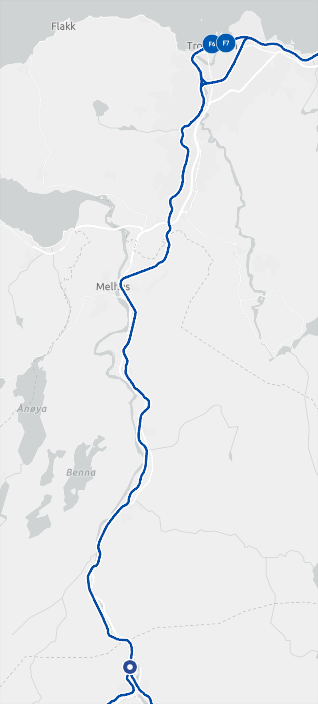
\includegraphics[scale=0.5]{figures/togkart.png}
    \caption{Map over train route from Trondheim to Støren}
    \label{fig:trainmap}
\end{figure}
\chapter{Confidentiality Contract}
\label{app:conf}

\begin{figure}[!h]
    \centering
    \includegraphics[scale=0.5]{figures/Jørgen F - CGF Data Access Agreement.pdf}
    \caption{Confidentiality contract with NTNU CGF}
    \label{fig:agreement}
\end{figure}

\end{document}
